\subsection{Künstliche Intelligenz}
Künstliche Intelligenz soll Computer in die Lage versetzen, Denkaufgaben zu erfüllen, zu denen Menschen und Tiere fähig sind.\newline
Allerdings können Computer bereits so erfolgreich und effizient programmiert werden, dass sie übermenschliche Fähigkeiten haben, um Probleme zu lösen und Spiele besser spielen als jeder Mensch \cite{10.5555/1795711}.\newline
Ein KI-Client ist daher im Folgenden der computergesteuerte Agent, der handelt. Er gilt nach \cite{Bartneck.2021} als intelligent, wenn... 
\begin{itemize}
    \item ...seine Handlungen den Umständen und Zielen angemessen sind. 
    \item ...er flexibel auf sich verändernde Umgebungen und Ziele reagieren kann.
    \item ...er aus Erfahrung lernt.
    \item ...er angesichts seiner Wahrnehmungs- und Berechnungsbeschränkungen angemessene Entscheidungen trifft.
\end{itemize}
In unserem Rennspiel soll also ein vom Computer gesteuerter Spieler die Steuerung eines Fahrzeuges und insbesondere das korrekte Abfahren der Rennstrecke übernehmen.\newline
Auf diese Weise erhält der Nutzer die Möglichkeit gegen den Computer Rennen zu fahren und sich mit diesem zu Messen.
Der KI-Client erhält dabei die gleichen Informationen zur Strecke wie der Nutzer und kommuniziert ferner auch auf die gleiche Weise mit dem Rennspiel und dessen abgekoppelten Rennspiellogik: mit einer der vier möglichen Richtungsentscheidungen \textit{oben}, \textit{unten}, \textit{links} oder \textit{rechts}.\newline
Darüber hinaus auch in kombinierter Form: \textit{oben+links}, \textit{oben+rechts}, \textit{unten+links} und \textit{unten+rechts}.\newline
In der nachfolgenden Abbildung \ref{fig:richtungen} sind die möglichen 8 Richtungen, die der Client auswählen und dem Rennspiel mitteilen kann, visualisiert.
\begin{figure}[h]
    \centering
    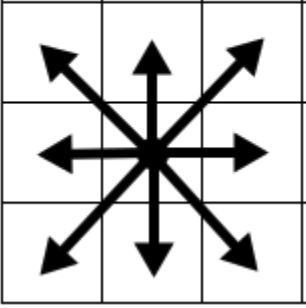
\includegraphics[scale=0.5]{pics/richtungen.png}
    \caption{Mögliche Richtungsentscheidungen der Clients mit dem jeweiligen Ausgangspunkt des Clients im mittleren Quadrat.}
    \label{fig:richtungen}
\end{figure}